% =====================================================================
%  Generative Scientific Discovery Engine -- technical report (submission)
%  Build:  tectonic submission_report.tex     (run from the docs/ folder)
%  Flowcharts are shared with project_guide.tex via figures/*.tex.
% =====================================================================
\documentclass[11pt,a4paper]{article}

\usepackage[T1]{fontenc}
\usepackage[utf8]{inputenc}
\usepackage{lmodern}
\usepackage[margin=2cm]{geometry}
\usepackage{amsmath,amssymb}
\usepackage{graphicx}
\usepackage{booktabs,array,tabularx}
\usepackage{enumitem}
\usepackage{xcolor}
\usepackage{tikz}
\usetikzlibrary{arrows.meta,positioning,shapes.geometric,shapes.misc,fit,backgrounds,calc}
\usepackage{float}
\usepackage{caption}
\usepackage{microtype}
\usepackage[hidelinks]{hyperref}
\usepackage[strings,nohyphen]{underscore}

\graphicspath{{../}}
\setlist{itemsep=1pt,topsep=3pt}
\setlength{\parskip}{3pt}
\setlength{\parindent}{0pt}
\captionsetup{font=small}
% Shared by project_guide.tex and submission_report.tex: macros, colours, flowchart styles, legend.
% Needs: xcolor, tikz (+ arrows.meta, positioning, shapes.geometric, shapes.misc, fit, backgrounds, calc),
% and the underscore package.

% ---------- code identifiers (underscores safe) ----------
\newcommand{\fn}[1]{\texttt{#1}}  % underscore pkg: _ prints literally and may break lines

% ---------- package colour palette (used in every flowchart) ----------
\definecolor{cData}{HTML}{6B7280}   % data/
\definecolor{cEqd}{HTML}{2563EB}    % equation_discovery/
\definecolor{cPinn}{HTML}{EA580C}   % pinn/
\definecolor{cVal}{HTML}{DC2626}    % validation/
\definecolor{cLlm}{HTML}{7C3AED}    % llm/
\definecolor{cHyp}{HTML}{15803D}    % hypotheses/
\definecolor{cRag}{HTML}{0D9488}    % rag/
\definecolor{cKg}{HTML}{92400E}     % knowledge_graph/
\definecolor{cEval}{HTML}{A16207}   % evaluation/
\definecolor{cExp}{HTML}{111827}    % experiments/

% ---------- flowchart styles ----------
\tikzset{
  >={Stealth[length=2.2mm]},
  fn/.style={draw=#1!75!black, fill=#1!10, rounded corners=2pt, line width=0.6pt,
             font=\ttfamily\scriptsize, align=center, inner sep=3pt, minimum height=6mm},
  fnw/.style={fn=#1, text width=47mm},
  stage/.style={draw=#1!75!black, fill=#1!8, rounded corners=3pt, line width=0.8pt,
                font=\small, align=left, inner sep=5pt, text width=0.80\textwidth},
  io/.style={draw=black!60, fill=black!4, font=\scriptsize\itshape, align=center,
             trapezium, trapezium left angle=75, trapezium right angle=105,
             inner sep=3pt, minimum height=6mm},
  dec/.style={draw=#1!75!black, fill=#1!10, diamond, aspect=2.4, font=\scriptsize,
              align=center, inner sep=1pt},
  note/.style={font=\scriptsize\itshape, text=black!65, align=left},
  flow/.style={->, line width=0.7pt, black!65},
  dflow/.style={->, line width=0.7pt, black!45, dashed},
  pkgbox/.style={draw=#1!60, fill=#1!4, rounded corners=4pt, line width=0.5pt, inner sep=6pt},
  pkglabel/.style={font=\ttfamily\scriptsize\bfseries, text=#1!80!black},
}

% legend used under every flowchart
\newcommand{\pkglegend}{%
  \par\smallskip\centering\scriptsize
  \tikz\node[fn=cData]{data};~\tikz\node[fn=cEqd]{equation\_discovery};~\tikz\node[fn=cPinn]{pinn};~%
  \tikz\node[fn=cVal]{validation};~\tikz\node[fn=cLlm]{llm};~\tikz\node[fn=cHyp]{hypotheses};\\[2pt]
  \tikz\node[fn=cRag]{rag};~\tikz\node[fn=cKg]{knowledge\_graph};~\tikz\node[fn=cEval]{evaluation};~%
  \tikz\node[fn=cExp]{experiments};\par}


\newcolumntype{L}[1]{>{\raggedright\arraybackslash}p{#1}}
\newcommand{\met}{\textbf{\color{green!50!black}Met}}
\newcommand{\partl}{\textbf{\color{orange!85!black}Partial}}
\newcommand{\notdone}{\textbf{\color{red!70!black}Not done}}

\title{\textbf{Generative Scientific Discovery Engine}\\[3pt]\large Technical Report}
\author{Namit Aggarwal}
\date{October 2026}

\begin{document}
\maketitle
\vspace{-6mm}

\begin{abstract}
\noindent Given 400 sparse, noisy observations of a field $u(x,t)$ and no governing equation, the system retrieves
scientific evidence (RAG + knowledge graph), generates candidate equations (LLM + graph templates), tests each with an
inverse physics-informed neural network (PINN), rejects invalid hypotheses on held-out data, selects the most
parsimonious supported law, and predicts beyond the observed window. It recovers $u_t = D\,u_{xx}$ with
$\hat D = 0.10002$ (truth 0.1), rejects advection and pure reaction, and predicts unseen times with RMSE
$2.5\times10^{-4}$, 40$\times$ better than a physics-free network. On a second, unseen system it recovers
$u_t + c\,u_x = D\,u_{xx}$ with both constants within 0.4\%. It passes 50/50 benchmark questions, 23/25 multi-hop
problems and 20/20 adversarial cases, and the pipeline also runs end to end with a real LLM (Google Gemini).
\end{abstract}

% =====================================================================
\section{System overview}
% =====================================================================

The pipeline follows the brief: \emph{Observed data $\to$ evidence $\to$ candidate physics $\to$ equation $\to$ PINN
$\to$ validation $\to$ new prediction} (Figure~\ref{fig:pipeline}). Division of responsibility is enforced in code:
RAG retrieves, the graph organises, the LLM only \emph{proposes}. Accept/reject and selection use only measured losses
on held-out noisy observations; the hidden truth is read in one function, after all decisions, to report error.

\begin{figure}[!tbp]
\centering
\scalebox{0.85}{% flowchart 'pipeline' -- used by docs/Report.tex
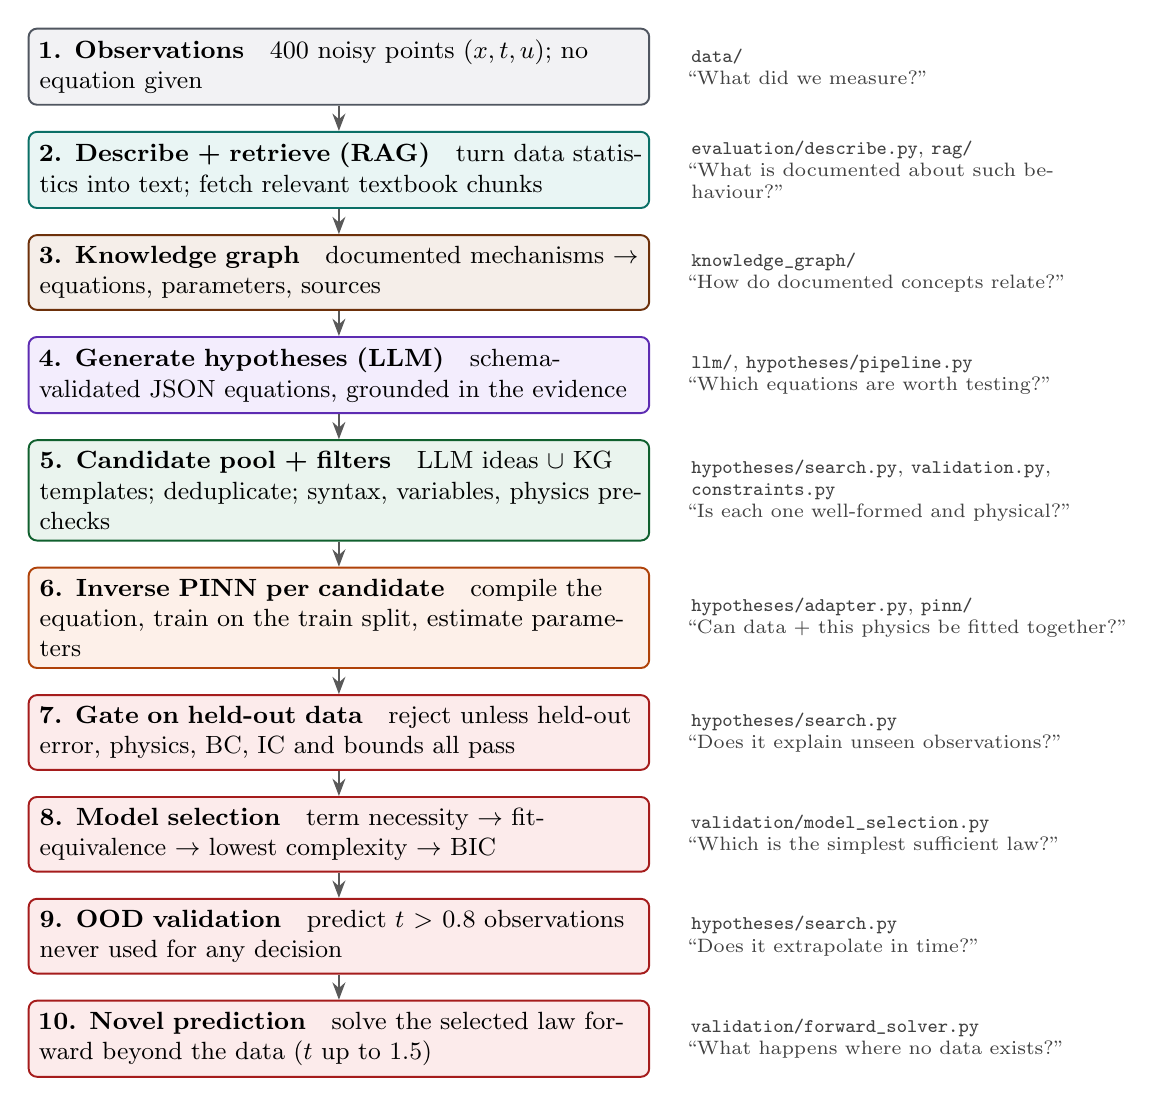
\begin{tikzpicture}[node distance=3.2mm]
  \tikzset{st/.style={draw=#1!75!black, fill=#1!9, rounded corners=3pt, line width=0.7pt,
                      font=\small, align=left, inner sep=4pt, text width=7.6cm},
           side/.style={font=\scriptsize, align=left, text width=5.6cm, text=black!75}}
  \node[st=cData] (s1) {\textbf{1. Observations}\quad 400 noisy points $(x,t,u)$; no equation given};
  \node[st=cRag, below=of s1] (s2) {\textbf{2. Describe + retrieve (RAG)}\quad turn data statistics into
        text; fetch relevant textbook chunks};
  \node[st=cKg, below=of s2] (s3) {\textbf{3. Knowledge graph}\quad documented mechanisms $\to$ equations,
        parameters, sources};
  \node[st=cLlm, below=of s3] (s4) {\textbf{4. Generate hypotheses (LLM)}\quad schema-validated JSON
        equations, grounded in the evidence};
  \node[st=cHyp, below=of s4] (s5) {\textbf{5. Candidate pool + filters}\quad LLM ideas $\cup$ KG templates;
        deduplicate; syntax, variables, physics pre-checks};
  \node[st=cPinn, below=of s5] (s6) {\textbf{6. Inverse PINN per candidate}\quad compile the equation, train
        on the train split, estimate parameters};
  \node[st=cVal, below=of s6] (s7) {\textbf{7. Gate on held-out data}\quad reject unless held-out error,
        physics, BC, IC and bounds all pass};
  \node[st=cVal, below=of s7] (s8) {\textbf{8. Model selection}\quad term necessity $\to$ fit-equivalence
        $\to$ lowest complexity $\to$ BIC};
  \node[st=cVal, below=of s8] (s9) {\textbf{9. OOD validation}\quad predict $t>0.8$ observations never used
        for any decision};
  \node[st=cVal, below=of s9] (s10) {\textbf{10. Novel prediction}\quad solve the selected law forward beyond
        the data ($t$ up to 1.5)};
  \foreach \a/\b in {s1/s2,s2/s3,s3/s4,s4/s5,s5/s6,s6/s7,s7/s8,s8/s9,s9/s10}
     \draw[flow] (\a) -- (\b);
  \node[side, right=4mm of s1]  {\fn{data/}\\ ``What did we measure?''};
  \node[side, right=4mm of s2]  {\fn{evaluation/describe.py}, \fn{rag/}\\ ``What is documented about such behaviour?''};
  \node[side, right=4mm of s3]  {\fn{knowledge_graph/}\\ ``How do documented concepts relate?''};
  \node[side, right=4mm of s4]  {\fn{llm/}, \fn{hypotheses/pipeline.py}\\ ``Which equations are worth testing?''};
  \node[side, right=4mm of s5]  {\fn{hypotheses/search.py}, \fn{validation.py}, \fn{constraints.py}\\ ``Is each one well-formed and physical?''};
  \node[side, right=4mm of s6]  {\fn{hypotheses/adapter.py}, \fn{pinn/}\\ ``Can data + this physics be fitted together?''};
  \node[side, right=4mm of s7]  {\fn{hypotheses/search.py}\\ ``Does it explain unseen observations?''};
  \node[side, right=4mm of s8]  {\fn{validation/model_selection.py}\\ ``Which is the simplest sufficient law?''};
  \node[side, right=4mm of s9]  {\fn{hypotheses/search.py}\\ ``Does it extrapolate in time?''};
  \node[side, right=4mm of s10] {\fn{validation/forward_solver.py}\\ ``What happens where no data exists?''};
\end{tikzpicture}
}
\caption{End-to-end pipeline. Colours mark the code package that implements each stage.}
\label{fig:pipeline}
\end{figure}

\textbf{Data.} Ground truth $u_t = 0.1\,u_{xx}$ on $x,t\in[0,1]$, zero boundary values,
$u(x,0)=\sin\pi x + 0.5\sin 3\pi x$. The system sees only 400 random points with 5\% Gaussian noise. Splits: train on
$t\le0.8$ (minus a random 20\% holdout used for the gate and selection); OOD $=$ all $t>0.8$, never used for any
decision; novel prediction on $t\in(1,1.5]$, where no data exists. All thresholds were fixed in \fn{config.yaml}
before each run.

% =====================================================================
\section{Requirement coverage}
% =====================================================================

\textbf{Minimum research challenge} (all met).
\begin{center}
\small
\begin{tabular}{@{}L{4.6cm}L{10.6cm}@{}}
\toprule
\textbf{Required} & \textbf{Delivered} \\ \midrule
$\ge$3 generated hypotheses & 5 candidates (mock run), 6 (Gemini run) \\
1 discovered governing equation & $u_t = D\,u_{xx}$, $\hat D = 0.10002$; and $u_t + 0.399\,u_x = 0.0201\,u_{xx}$ on a second system \\
1 inverse / 1 forward PINN & Phase 3 (both), every Phase 6 candidate is an inverse PINN \\
1 sparse/noisy experiment & all main experiments use 400 points with 5\% noise \\
1 OOD prediction & $t>0.8$: RMSE 0.0018 vs clean field; novel $t\in(1,1.5]$: $2.5\times10^{-4}$ \\
1 correctly rejected hypothesis & advection (holdout RMSE 0.227 vs gate 0.03) and pure reaction (0.118) \\
20 adversarial physics cases & 20/20 (3 by abstention) \\
\bottomrule
\end{tabular}
\end{center}

\begin{center}
\small
\begin{tabular}{@{}L{4.6cm}L{8.6cm}l@{}}
\multicolumn{3}{@{}l}{\normalsize\textbf{Mandatory research components}}\\[3pt]
\toprule
\textbf{Mandatory component} & \textbf{Implementation and evidence} & \textbf{Status} \\ \midrule
Scientific RAG + knowledge graph & \fn{rag/}, \fn{knowledge_graph/}; 22 entities, 40 relationships, all with provenance & \met \\
Generative hypotheses from multi-source evidence & LLM proposals $\cup$ graph templates (\fn{hypotheses/search.py}); mock and real Gemini runs & \met \\
PINN forward and inverse & \fn{pinn/}; forward RMSE $7.3\times10^{-4}$; inverse $\hat D$ error 0.11\% & \met \\
PDE/ODE discovery from data & SINDy (\fn{equation_discovery/}) on clean/sparse data; PINN-based identification on noisy data & \partl \\
Unknown parameter estimation (PINN) & $D$ within 0.02\%; $c, D$ within 0.4\% on a second system & \met \\
Sparse/noisy-data learning & 400 points, 5\% noise, two systems & \met \\
Boundary/initial-condition inference & BC/IC supplied as known physics; enforced and checked, not inferred & \notdone \\
Physics-constrained generative search & bounds ($D,K>0$), well-posedness pre-checks, PINN gate (Figures~\ref{fig:p6}--\ref{fig:selection}) & \met \\
Uncertainty estimation & bootstrap coefficient stability (20 subsets); not Bayesian & \partl \\
Out-of-distribution validation & held-out $t>0.8$ and novel window $t\in(1,1.5]$ & \met \\
Comparison with NN and numerical solver & same network without physics; RK4/Euler forward solver & \met \\
\bottomrule
\end{tabular}
\end{center}


% =====================================================================
\section{Method: physics-constrained generative search}
% =====================================================================

\begin{enumerate}
  \item \textbf{Evidence.} The observations are summarised as text (statistics only, never naming a mechanism) and used
        to query a 5-document corpus; the knowledge graph returns the documented equations and parameters. A check
        confirms the corpus never states the dataset's parameter values (no answer leakage).
  \item \textbf{Generation.} The LLM returns schema-validated JSON hypotheses; graph templates are added; structural
        duplicates are removed (parameter- and sign-invariant signatures).
  \item \textbf{Pre-checks.} Syntax, variables, parameters, declared vs.\ actual derivatives, unit metadata, evolution
        form, physical bounds, boundary-condition well-posedness.
  \item \textbf{Inverse PINN per candidate.} Each equation string is compiled by SymPy into the residual of one shared
        PINN (4$\times$64 tanh, Adam 3000 + L-BFGS 300); unknown parameters train jointly with the network.
  \item \textbf{Gate} (held-out noisy data): holdout RMSE $\le0.03$, physics residual $\le0.01$, BC loss $\le0.005$,
        IC loss $\le0.01$, physical bounds.
  \item \textbf{Selection} (Figure~\ref{fig:selection}): fit-equivalence (within 5\% of best) $\to$ drop inactive terms
        ($<$5\% of $u_t$) $\to$ lowest complexity $\to$ BIC.
  \item \textbf{Validation and prediction.} Bootstrap stability, conservation check, OOD prediction, and a forward solve
        of the selected law beyond the data.
\end{enumerate}

\begin{figure}[p]
\centering
% flowchart 'p6' -- shared by project_guide.tex and submission_report.tex
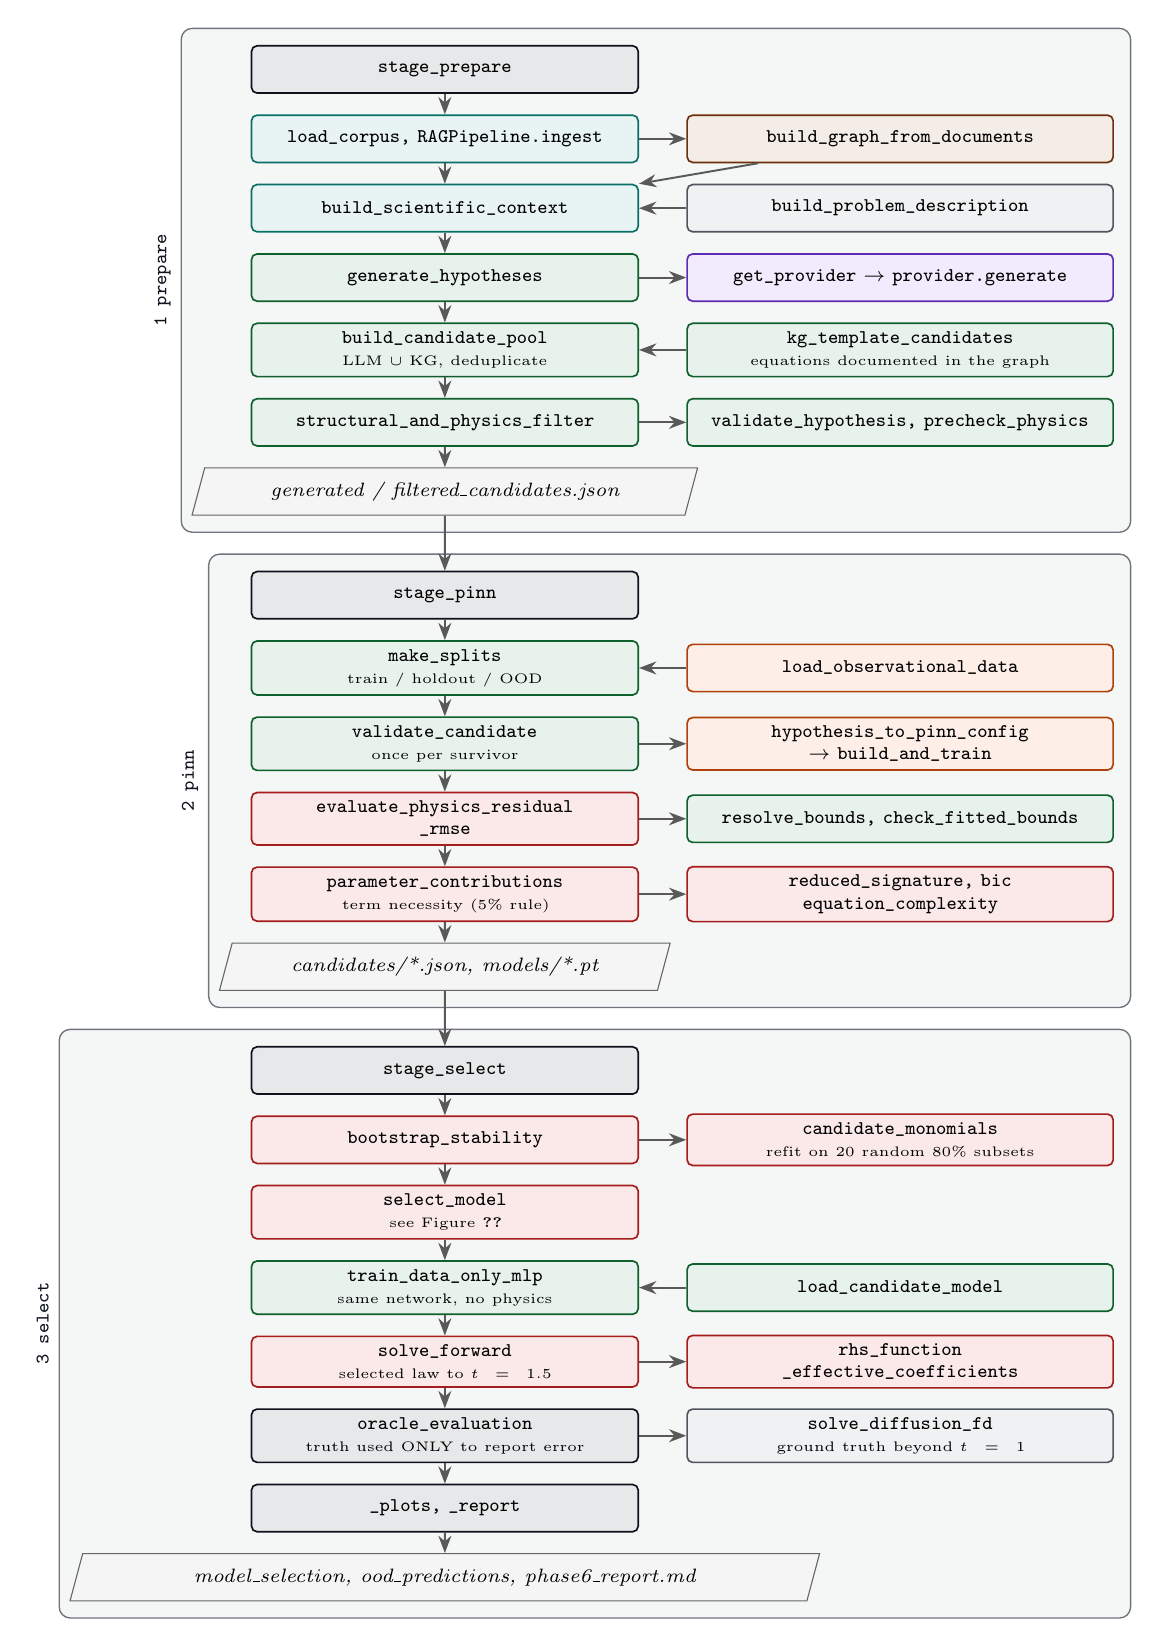
\begin{tikzpicture}[node distance=2.6mm and 6mm]
  \tikzset{sp/.style={fnw=#1}, hp/.style={fnw=#1, text width=52mm}}
  % ---------------- stage 1 ----------------
  \node[sp=cExp] (p0) {stage_prepare};
  \node[sp=cRag, below=of p0] (p1) {load_corpus, RAGPipeline.ingest};
  \node[hp=cKg, right=of p1] (h1) {build_graph_from_documents};
  \node[sp=cRag, below=of p1] (p2) {build_scientific_context};
  \node[hp=cData, right=of p2] (h2) {build_problem_description};
  \node[sp=cHyp, below=of p2] (p3) {generate_hypotheses};
  \node[hp=cLlm, right=of p3] (h3) {get_provider $\to$ provider.generate};
  \node[sp=cHyp, below=of p3] (p4) {build_candidate_pool\\{\normalfont\tiny LLM $\cup$ KG, deduplicate}};
  \node[hp=cHyp, right=of p4] (h4) {kg_template_candidates\\{\normalfont\tiny equations documented in the graph}};
  \node[sp=cHyp, below=of p4] (p5) {structural_and_physics_filter};
  \node[hp=cHyp, right=of p5] (h5) {validate_hypothesis, precheck_physics};
  \node[io, below=of p5] (o1) {generated / filtered\_candidates.json};
  % ---------------- stage 2 ----------------
  \node[sp=cExp, below=7mm of o1] (q0) {stage_pinn};
  \node[sp=cHyp, below=of q0] (q1) {make_splits\\{\normalfont\tiny train / holdout / OOD}};
  \node[hp=cPinn, right=of q1] (g1) {load_observational_data};
  \node[sp=cHyp, below=of q1] (q2) {validate_candidate\\{\normalfont\tiny once per survivor}};
  \node[hp=cPinn, right=of q2] (g2) {hypothesis_to_pinn_config\\$\to$ build_and_train};
  \node[sp=cVal, below=of q2] (q3) {evaluate_physics_residual\\_rmse};
  \node[hp=cHyp, right=of q3] (g3) {resolve_bounds, check_fitted_bounds};
  \node[sp=cVal, below=of q3] (q4) {parameter_contributions\\{\normalfont\tiny term necessity (5\% rule)}};
  \node[hp=cVal, right=of q4] (g4) {reduced_signature, bic\\equation_complexity};
  \node[io, below=of q4] (o2) {candidates/*.json, models/*.pt};
  % ---------------- stage 3 ----------------
  \node[sp=cExp, below=7mm of o2] (r0) {stage_select};
  \node[sp=cVal, below=of r0] (r1) {bootstrap_stability};
  \node[hp=cVal, right=of r1] (k1) {candidate_monomials\\{\normalfont\tiny refit on 20 random 80\% subsets}};
  \node[sp=cVal, below=of r1] (r2) {select_model\\{\normalfont\tiny see Figure \ref{fig:selection}}};
  \node[sp=cHyp, below=of r2] (r3) {train_data_only_mlp\\{\normalfont\tiny same network, no physics}};
  \node[hp=cHyp, right=of r3] (k3) {load_candidate_model};
  \node[sp=cVal, below=of r3] (r4) {solve_forward\\{\normalfont\tiny selected law to $t=1.5$}};
  \node[hp=cVal, right=of r4] (k4) {rhs_function\\_effective_coefficients};
  \node[sp=cExp, below=of r4] (r5) {oracle_evaluation\\{\normalfont\tiny truth used ONLY to report error}};
  \node[hp=cData, right=of r5] (k5) {solve_diffusion_fd\\{\normalfont\tiny ground truth beyond $t=1$}};
  \node[sp=cExp, below=of r5] (r6) {_plots, _report};
  \node[io, below=of r6] (o3) {model\_selection, ood\_predictions, phase6\_report.md};
  % groups
  \begin{scope}[on background layer]
    \node[pkgbox=cExp, fit=(p0)(h1)(h5)(o1), label={[pkglabel=cExp]left:\rotatebox{90}{1 prepare}}] {};
    \node[pkgbox=cExp, fit=(q0)(g1)(g4)(o2), label={[pkglabel=cExp]left:\rotatebox{90}{2 pinn}}] {};
    \node[pkgbox=cExp, fit=(r0)(k1)(k5)(o3), label={[pkglabel=cExp]left:\rotatebox{90}{3 select}}] {};
  \end{scope}
  % arrows
  \foreach \a/\b in {p0/p1,p1/p2,p2/p3,p3/p4,p4/p5,p5/o1,o1/q0,q0/q1,q1/q2,q2/q3,q3/q4,q4/o2,o2/r0,r0/r1,r1/r2,r2/r3,r3/r4,r4/r5,r5/r6,r6/o3}
    \draw[flow] (\a) -- (\b);
  \foreach \a/\b in {p1/h1,h2/p2,p3/h3,h4/p4,p5/h5,g1/q1,q2/g2,q3/g3,q4/g4,r1/k1,k3/r3,r4/k4,r5/k5}
    \draw[flow] (\a) -- (\b);
  \draw[flow] (h1) -- (p2.north east);
\end{tikzpicture}

\pkglegend
\caption{Function-level flow of the search (\fn{experiments/08_physics_constrained_search.py}), stage by stage.
Only \fn{oracle_evaluation} reads the ground truth, after all decisions.}
\label{fig:p6}
\end{figure}

\begin{figure}[!htb]
\centering
% flowchart 'selection' -- used by docs/Report.tex
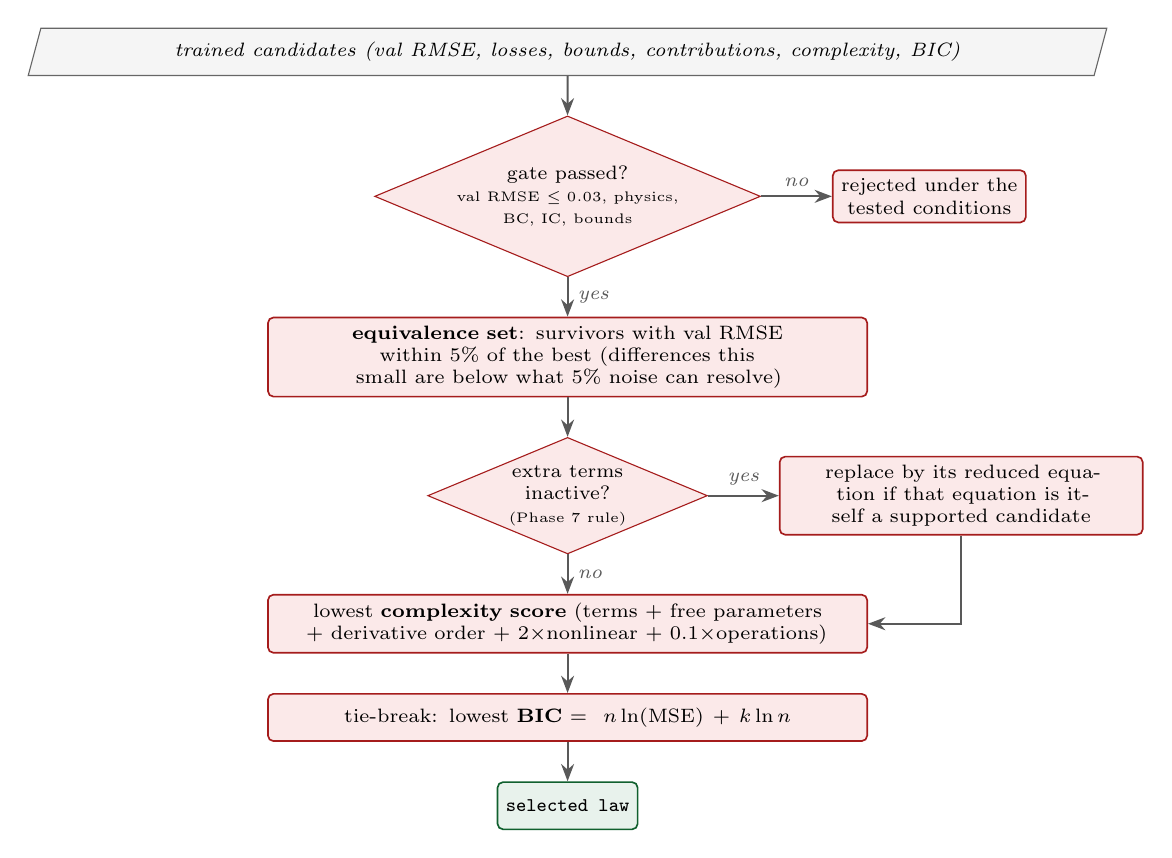
\begin{tikzpicture}[node distance=5mm and 9mm]
  \node[io] (in) {trained candidates (val RMSE, losses, bounds, contributions, complexity, BIC)};
  \node[dec=cVal, below=of in] (g) {gate passed?\\{\tiny val RMSE $\le 0.03$, physics,}\\{\tiny BC, IC, bounds}};
  \node[fn=cVal, font=\scriptsize, right=of g] (rej) {rejected under the\\tested conditions};
  \node[fn=cVal, font=\scriptsize, below=of g, text width=74mm] (eq) {\textbf{equivalence set}: survivors with val RMSE within 5\% of the best
        (differences this small are below what 5\% noise can resolve)};
  \node[dec=cVal, below=of eq] (red) {extra terms\\inactive?\\{\tiny (Phase 7 rule)}};
  \node[fn=cVal, font=\scriptsize, right=of red, text width=44mm] (rd) {replace by its reduced equation if that equation is
        itself a supported candidate};
  \node[fn=cVal, font=\scriptsize, below=of red, text width=74mm] (cx) {lowest \textbf{complexity score}
        (terms + free parameters + derivative order + 2$\times$nonlinear + 0.1$\times$operations)};
  \node[fn=cVal, font=\scriptsize, below=of cx, text width=74mm] (bic) {tie-break: lowest \textbf{BIC} $= n\ln(\mathrm{MSE}) + k\ln n$};
  \node[fn=cHyp, below=of bic] (sel) {\textbf{selected law}};
  \draw[flow] (in) -- (g);
  \draw[flow] (g) -- node[note, above]{no} (rej);
  \draw[flow] (g) -- node[note, right]{yes} (eq);
  \draw[flow] (eq) -- (red);
  \draw[flow] (red) -- node[note, above]{yes} (rd);
  \draw[flow] (rd) |- (cx.east);
  \draw[flow] (red) -- node[note, right]{no} (cx);
  \draw[flow] (cx) -- (bic); \draw[flow] (bic) -- (sel);
\end{tikzpicture}

\caption{Model-selection rule (\fn{validation/model_selection.py}); thresholds fixed before any run.}
\label{fig:selection}
\end{figure}

\textbf{Ranking criteria requested by the brief, and where each is used:}
\begin{center}
\small
\begin{tabular}{@{}L{3.3cm}L{9.0cm}L{3.0cm}@{}}
\toprule
\textbf{Criterion} & \textbf{Measure} & \textbf{Used in} \\ \midrule
Data fit & holdout RMSE on noisy observations & gate, equivalence \\
PDE residual & mean squared residual on a fresh grid & gate \\
Conservation laws & global balance violation $\mathrm{RMS}_t\!\int\!\mathcal R\,dx \,/\, \mathrm{RMS}_t\, dM/dt$ & reported \\
Dimensional consistency & declared units per parameter (fraction complete) & pre-check (metadata) \\
Boundary/initial conditions & BC and IC losses; well-posedness warnings & gate, pre-check \\
Complexity & terms + parameters + derivative order + 2$\times$nonlinear + 0.1$\times$ops & selection \\
Uncertainty & bootstrap coefficient mean, spread, sign stability & reported \\
\bottomrule
\end{tabular}
\end{center}

% =====================================================================
\section{Results}
% =====================================================================

\subsection{Hypothesis testing and the discovered law}

\begin{center}
\footnotesize
\setlength{\tabcolsep}{3.5pt}
\begin{tabular}{@{}llllllr@{}}
\toprule
\textbf{ID} & \textbf{Candidate} & \textbf{Estimates} & \textbf{Holdout} & \textbf{Status} & \textbf{Inactive} & \textbf{Cons.\ viol.} \\ \midrule
H1 & $u_t = D\,u_{xx}$ & $D=0.10002$ & 0.01214 & \textbf{selected} & -- & 0.08\% \\
H2 & $u_t + c\,u_x = 0$ & $c=0.0089$ & 0.2269 & rejected & -- & 100\% \\
H3 & $u_t = D\,u_{xx} + r\,u(1-u/K)$ & $D{=}0.101, r{=}0.023, K{=}1.18$ & 0.01217 & supported & $r, K$ & 0.11\% \\
H4 & $u_t + c\,u_x = D\,u_{xx}$ & $c{=}{-0.0002}, D{=}0.09995$ & 0.01214 & supported & $c$ & 0.13\% \\
K3 & $u_t = r\,u(1-u/K)$ (graph) & $r{=}{-1.44}, K{=}6.67$ & 0.1176 & rejected & -- & 0.75\% \\
\bottomrule
\end{tabular}
\end{center}

H1, H3 and H4 fit to the noise floor ($\approx0.012$); H3 and H4 carry inactive terms and reduce to H1, which has the
lowest complexity, and BIC agrees. A pure best-fit rule would have chosen H4 (lower by 0.06\%). Advection breaks global
conservation completely: with zero boundary values it conserves $\int u\,dx$, while the data loses it.

\subsection{PINN research results}

\begin{center}
\footnotesize
\begin{tabular}{@{}L{3.6cm}L{3.3cm}L{3.3cm}L{5.0cm}@{}}
\toprule
\textbf{Metric} & \textbf{Forward ($D$ fixed)} & \textbf{Inverse ($D$ from 0.2)} & \textbf{Phase 6 selected (H1)} \\ \midrule
PDE residual (fresh grid) & $2.7\times10^{-5}$ & $3.3\times10^{-5}$ & $1.4\times10^{-5}$ \\
Data loss & $1.32\times10^{-4}$ & $1.32\times10^{-4}$ & $1.29\times10^{-4}$ \\
Boundary / initial loss & $2.4\times10^{-6}$ / $8\times10^{-7}$ & $2.8\times10^{-6}$ / $1.2\times10^{-6}$ & $1.0\times10^{-6}$ / $1.0\times10^{-6}$ \\
Parameter error & -- & 0.11\% & 0.02\% \\
Prediction error (vs clean) & RMSE $7.3\times10^{-4}$ & RMSE $8.8\times10^{-4}$ & OOD RMSE $1.8\times10^{-3}$ \\
Conservation violation & -- & -- & 0.08\% (train), 1.7\% (OOD), 5.6\% ($t>1$) \\
Uncertainty (bootstrap $u_{xx}$ coef.) & -- & -- & $0.110\pm0.003$, sign-stable 100\% \\
OOD (noisy holdout, $t>0.8$) & -- & -- & RMSE 0.0114 (noise floor $\approx0.012$) \\
\bottomrule
\end{tabular}
\end{center}
The bootstrap uses finite-difference derivatives and is biased high (0.110 vs.\ the PINN's 0.100); it measures term
stability, not a calibrated interval.

\subsection{Comparison with a conventional network and a numerical solver}

\begin{center}
\small
\begin{tabular}{@{}L{5.4cm}L{5.4cm}L{4.6cm}@{}}
\toprule
\textbf{Model} & \textbf{OOD RMSE, $t>0.8$ (vs clean)} & \textbf{Conservation viol.\ (train / OOD)} \\ \midrule
PINN, selected law H1 & 0.0018 & 0.08\% / 1.7\% \\
Same network, data only (no physics) & 0.0712 (40$\times$ worse) & 15\% / 5.3\% \\
Forward solver (RK4) with $\hat D$, no data & 0.0003; novel $t\in(1,1.5]$: 0.00025 & -- \\
\bottomrule
\end{tabular}
\end{center}

\subsection{Sparse/noisy data and generalisation}

SINDy recovers $u_t = 0.1009\,u_{xx}$ (clean) and $0.1013\,u_{xx}$ (sparse) but fails on the 400 noisy points
(five spurious terms); the PINN path succeeds on the same data. On a second hidden system
($u_t + 0.4\,u_x = 0.02\,u_{xx}$, $x\in[0,1.5]$, Gaussian start, 400 points, 5\% noise) the identical pipeline rejects
diffusion, advection and reaction--diffusion and selects advection--diffusion with $c=0.39897$, $D=0.02008$ (errors
0.26\%, 0.40\%), OOD RMSE 0.0010 vs.\ 0.0068 for the physics-free network, and 0.58\% error beyond the data window.
SINDy on that data returned a spurious equation.

\subsection{Real LLM (Gemini)}

With \fn{gemini-3.5-flash-lite} (larger models were overloaded), retrieved evidence changed the generated hypotheses on
all three test datasets. In the full search Gemini proposed $D u_{xx}$, $D u_{xx} - r u$, advection--diffusion and
reaction--diffusion; the graph added pure advection and pure reaction, which were rejected. The same law was selected
($\hat D = 0.10001$, OOD RMSE 0.0020 vs.\ clean). This is a single sample of a stochastic generator.

% =====================================================================
\section{Benchmark and ablation}
% =====================================================================

Twelve benchmark datasets (diffusion, advection, reaction--diffusion, advection--diffusion; 3 settings each).
\textbf{50 questions: 50/50}; \textbf{25 multi-hop problems: 23/25} (both failures from top-1 lexical retrieval);
\textbf{20 adversarial cases: 20/20}, including invalid equations, negative diffusivity, time-reversed data, disguised
duplicates, malicious LLM output, a non-identifiable dataset, Occam traps, answer leakage and prompt injection (three
noise/sparsity cases pass by abstention).

\begin{center}
\small
\begin{tabular}{@{}lcc@{}}
\toprule
\textbf{Ablation arm} (12 datasets) & \textbf{Correct law} & \textbf{OOD within 5\%} \\ \midrule
LLM/RAG generation, no validation & 3/12 & 3/12 \\
RAG + KG generation, no validation & 3/12 & 3/12 \\
Equation discovery alone (SINDy) & 8/12 & 6/12 \\
\textbf{Full system} (generation + physics validation + selection) & \textbf{12/12} & \textbf{12/12} \\
Full system without the LLM & 12/12 & 12/12 \\
\bottomrule
\end{tabular}
\end{center}
Physics validation and selection drive accuracy; RAG supplies a candidate pool containing the truth (top-1 retrieval
only 1/6); the graph and mock LLM add no measurable accuracy here. A leakage audit confirms no decision function
reads ground truth and catches a planted cheating selector.

% =====================================================================
\section{Limitations}
% =====================================================================
\begin{itemize}
  \item Synthetic 1-D PDEs only; known laws recovered, no new law claimed.
  \item Boundary/initial conditions are given, not inferred.
  \item Uncertainty is a bootstrap of term stability, not a Bayesian posterior.
  \item Nested models fit equally well; selection relies on a stated parsimony rule, not uniqueness.
  \item Lexical retrieval over a 5-document corpus; thresholds hand-set (fixed in advance, not calibrated).
  \item Conservation is a consistency check, not a discriminator: a network fitted to a wrong law can still follow
        that law (K3: 0.75\%), so it is reported alongside the data gate rather than replacing it.
\end{itemize}

% =====================================================================
\section{Deliverables and reproducibility}
% =====================================================================
\begin{center}
\small
\begin{tabular}{@{}L{3.6cm}L{12.0cm}@{}}
\toprule
\textbf{Artifact} & \textbf{Location} \\ \midrule
Code & \fn{data/}, \fn{equation_discovery/}, \fn{pinn/}, \fn{validation/}, \fn{llm/}, \fn{hypotheses/}, \fn{rag/},
        \fn{knowledge_graph/}, \fn{evaluation/}; 95 tests in \fn{tests/} \\
Datasets & \fn{data/generated/*.npz} (clean, sparse, noisy, benchmark, second system) \\
Trained models & \fn{results/phase6/models/}, \fn{results/evaluation/generalization/models/} \\
Discovered equations & \fn{results/phase6/model_selection.json}, \fn{.../generalization/generalization_results.json} \\
Knowledge graph & \fn{results/rag_kg/knowledge_graph.json} \\
Experiments & \fn{experiments/02}--\fn{12} (one script per phase) \\
Benchmark & \fn{results/evaluation/} (questions, multi-hop, adversarial, ablation, leakage) \\
Conservation; Gemini run & \fn{results/evaluation/conservation/}; \fn{results/evaluation/real_llm_gemini/} \\
Reports & this report; \fn{results/final_report.md}; \fn{docs/project_guide.pdf} (detailed guide) \\
\bottomrule
\end{tabular}
\end{center}

\textbf{Reproduce:} install with \fn{pip install -r requirements.txt} and test with \fn{python -m pytest tests}.
Then run \fn{data/generate_diffusion.py} and the experiment scripts 02--12 in order, each with
\fn{-{}-config config.yaml} (each PINN takes about 4 minutes on CPU; stages are cached). The Gemini run needs \fn{GEMINI_API_KEY}; see \fn{README.md}.

% =====================================================================
\appendix
\section{Additional flowcharts}
% =====================================================================
Function-level flows of the remaining components. Colours follow the package legend.

\begin{figure}[!htb]\centering% flowchart 'packages' -- used by docs/Report.tex
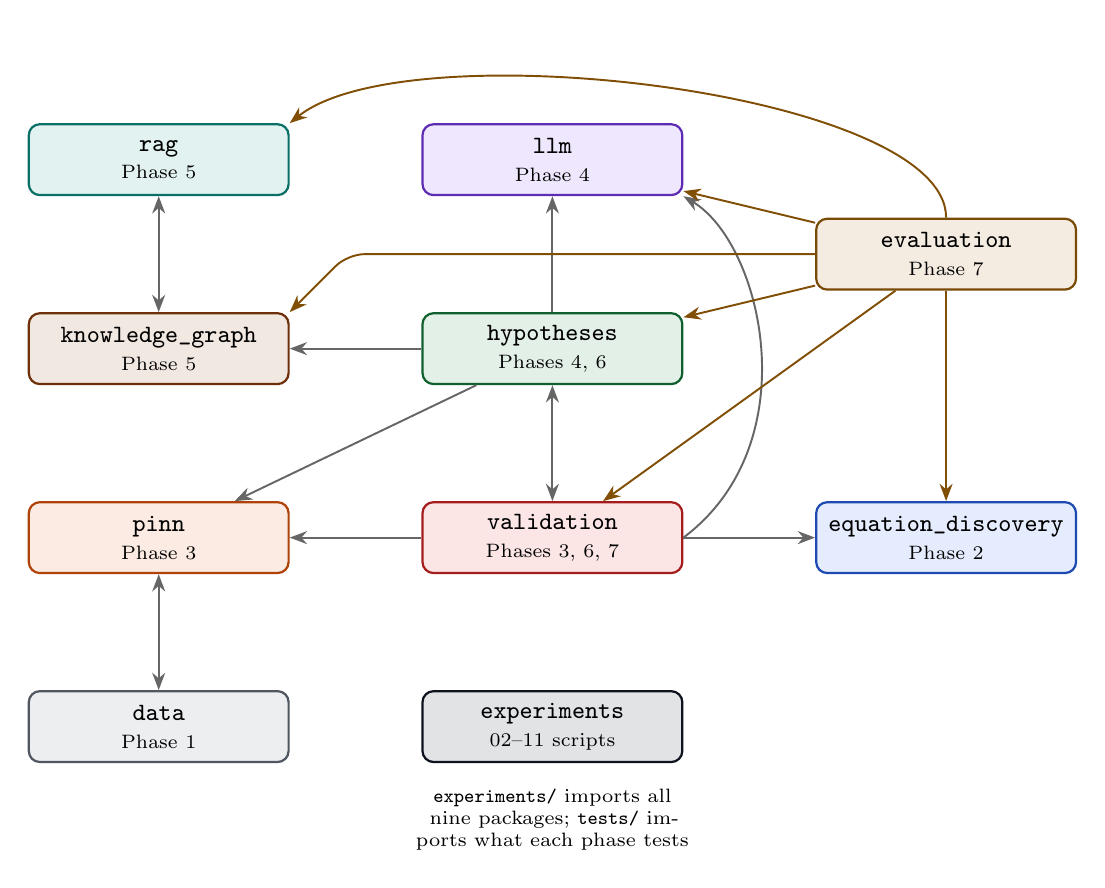
\begin{tikzpicture}[
   pk/.style={draw=#1!75!black, fill=#1!12, rounded corners=4pt, line width=0.8pt,
              font=\ttfamily\small\bfseries, minimum width=3.3cm, minimum height=9mm, align=center},
   dep/.style={->, line width=0.7pt, black!60},
   mdep/.style={<->, line width=0.7pt, black!60}]
  \node[pk=cRag]  (rag) at (0,0)     {rag\\[-1pt]{\normalfont\scriptsize Phase 5}};
  \node[pk=cKg]   (kg)  at (0,-2.4)  {knowledge\_graph\\[-1pt]{\normalfont\scriptsize Phase 5}};
  \node[pk=cLlm]  (llm) at (5,0)     {llm\\[-1pt]{\normalfont\scriptsize Phase 4}};
  \node[pk=cHyp]  (hyp) at (5,-2.4)  {hypotheses\\[-1pt]{\normalfont\scriptsize Phases 4, 6}};
  \node[pk=cVal]  (val) at (5,-4.8)  {validation\\[-1pt]{\normalfont\scriptsize Phases 3, 6, 7}};
  \node[pk=cPinn] (pinn) at (0,-4.8) {pinn\\[-1pt]{\normalfont\scriptsize Phase 3}};
  \node[pk=cData] (data) at (0,-7.2) {data\\[-1pt]{\normalfont\scriptsize Phase 1}};
  \node[pk=cEqd]  (eqd) at (10,-4.8) {equation\_discovery\\[-1pt]{\normalfont\scriptsize Phase 2}};
  \node[pk=cEval] (ev)  at (10,-1.2) {evaluation\\[-1pt]{\normalfont\scriptsize Phase 7}};
  \node[pk=cExp]  (exp) at (5,-7.2)  {experiments\\[-1pt]{\normalfont\scriptsize 02--11 scripts}};

  \draw[mdep] (rag) -- (kg);
  \draw[mdep] (pinn) -- (data);
  \draw[mdep] (hyp) -- (val);
  \draw[dep] (hyp) -- (kg);
  \draw[dep] (hyp) -- (llm);
  \draw[dep] (hyp) -- (pinn);
  \draw[dep] (val) -- (pinn);
  \draw[dep] (val) -- (eqd);
  \draw[dep] (val.east) .. controls +(1.6,1.2) and +(1.0,-0.6) .. (llm.south east);
  \draw[dep, cEval!80!black] (ev) -- (llm);
  \draw[dep, cEval!80!black] (ev) -- (hyp);
  \draw[dep, cEval!80!black] (ev) -- (eqd);
  \draw[dep, cEval!80!black] (ev) -- (val);
  \draw[dep, cEval!80!black] (ev.north) .. controls +(0,1.6) and +(1.5,1.2) .. (rag.north east);
  \draw[dep, cEval!80!black, rounded corners=6pt] (ev.west) -- (2.4,-1.2) -- (kg.north east);
  \node[font=\scriptsize, align=center, text width=4.4cm, below=2mm of exp]
       {\fn{experiments/} imports all nine packages; \fn{tests/} imports what each phase tests};
\end{tikzpicture}

\caption{Package dependency map (from the actual imports).}\end{figure}

\begin{figure}[!htb]\centering% flowchart 'p2' -- used by docs/Report.tex
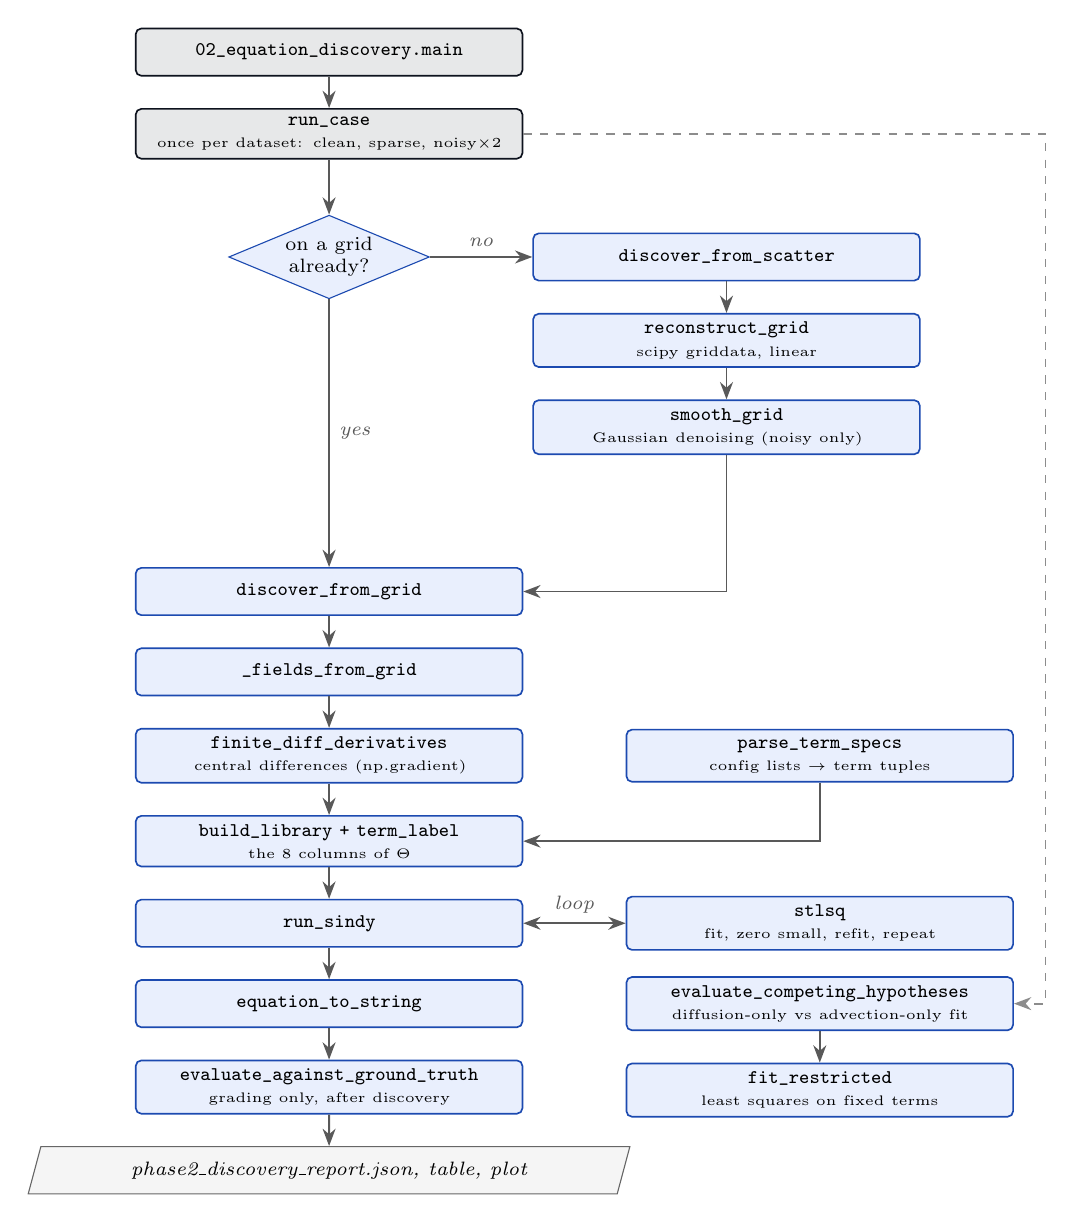
\begin{tikzpicture}[node distance=4mm and 7mm]
  \node[fnw=cExp] (main) {02_equation_discovery.main};
  \node[fnw=cExp, below=of main] (case) {run_case\\{\normalfont\tiny once per dataset: clean, sparse, noisy$\times$2}};
  \node[dec=cEqd, below=7mm of case] (q) {on a grid\\already?};
  \node[fnw=cEqd, right=of q, xshift=6mm] (scat) {discover_from_scatter};
  \node[fnw=cEqd, below=of scat] (rec) {reconstruct_grid\\{\normalfont\tiny scipy griddata, linear}};
  \node[fnw=cEqd, below=of rec] (sm) {smooth_grid\\{\normalfont\tiny Gaussian denoising (noisy only)}};
  \node[fnw=cEqd, below=34mm of q] (grid) {discover_from_grid};
  \node[fnw=cEqd, below=of grid] (fields) {_fields_from_grid};
  \node[fnw=cEqd, below=of fields] (fdd) {finite_diff_derivatives\\{\normalfont\tiny central differences (np.gradient)}};
  \node[fnw=cEqd, right=of fdd, xshift=6mm] (specs) {parse_term_specs\\{\normalfont\tiny config lists $\to$ term tuples}};
  \node[fnw=cEqd, below=of fdd] (lib) {build_library + term_label\\{\normalfont\tiny the 8 columns of $\Theta$}};
  \node[fnw=cEqd, below=of lib] (sindy) {run_sindy};
  \node[fnw=cEqd, right=of sindy, xshift=6mm] (stlsq) {stlsq\\{\normalfont\tiny fit, zero small, refit, repeat}};
  \node[fnw=cEqd, below=of sindy] (str) {equation_to_string};
  \node[fnw=cEqd, below=of str] (gt) {evaluate_against_ground_truth\\{\normalfont\tiny grading only, after discovery}};
  \node[fnw=cEqd, right=of str, xshift=6mm] (comp) {evaluate_competing_hypotheses\\{\normalfont\tiny diffusion-only vs advection-only fit}};
  \node[fnw=cEqd, below=of comp] (restr) {fit_restricted\\{\normalfont\tiny least squares on fixed terms}};
  \node[io, below=of gt] (out) {phase2\_discovery\_report.json, table, plot};
  \draw[flow] (main) -- (case); \draw[flow] (case) -- (q);
  \draw[flow] (q) -- node[note, above]{no} (scat);
  \draw[flow] (q) -- node[note, right]{yes} (grid);
  \draw[flow] (scat) -- (rec); \draw[flow] (rec) -- (sm); \draw[flow] (sm) |- (grid);
  \draw[flow] (grid) -- (fields); \draw[flow] (fields) -- (fdd); \draw[flow] (fdd) -- (lib);
  \draw[flow] (specs) |- (lib);
  \draw[flow] (lib) -- (sindy); \draw[flow, <->] (sindy) -- node[note, above]{loop} (stlsq);
  \draw[flow] (sindy) -- (str); \draw[flow] (str) -- (gt); \draw[flow] (gt) -- (out);
  \draw[dflow] (case.east) -| ([xshift=4mm]comp.east) -- (comp.east);
  \draw[flow] (comp) -- (restr);
\end{tikzpicture}
\pkglegend
\caption{PDE discovery from data (SINDy/STLSQ).}\end{figure}

\begin{figure}[!htb]\centering% flowchart 'p3' -- used by docs/Report.tex
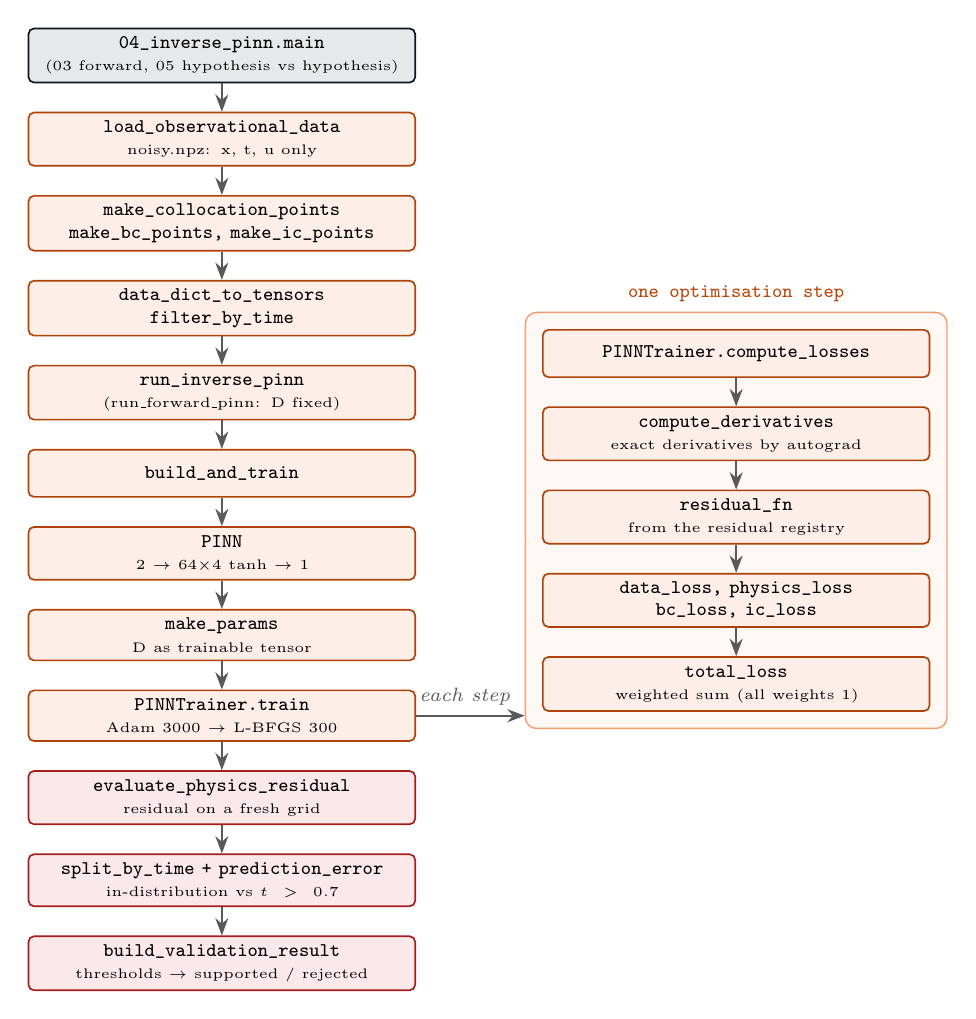
\begin{tikzpicture}[node distance=3.6mm and 6mm]
  % left column: experiment set-up
  \node[fnw=cExp] (main) {04_inverse_pinn.main\\{\normalfont\tiny (03 forward, 05 hypothesis vs hypothesis)}};
  \node[fnw=cPinn, below=of main] (load) {load_observational_data\\{\normalfont\tiny noisy.npz: x, t, u only}};
  \node[fnw=cPinn, below=of load] (pts) {make_collocation_points\\make_bc_points, make_ic_points};
  \node[fnw=cPinn, below=of pts] (tens) {data_dict_to_tensors\\filter_by_time};
  \node[fnw=cPinn, below=of tens] (inv) {run_inverse_pinn\\{\normalfont\tiny (run\_forward\_pinn: D fixed)}};
  \node[fnw=cPinn, below=of inv] (bt) {build_and_train};
  \node[fnw=cPinn, below=of bt] (net) {PINN\\{\normalfont\tiny 2 $\to$ 64$\times$4 tanh $\to$ 1}};
  \node[fnw=cPinn, below=of net] (mp) {make_params\\{\normalfont\tiny D as trainable tensor}};
  \node[fnw=cPinn, below=of mp] (tr) {PINNTrainer.train\\{\normalfont\tiny Adam 3000 $\to$ L-BFGS 300}};
  % right column: one loss evaluation
  \node[fnw=cPinn, right=of tr, xshift=10mm, yshift=46mm] (cl) {PINNTrainer.compute_losses};
  \node[fnw=cPinn, below=of cl] (cd) {compute_derivatives\\{\normalfont\tiny exact derivatives by autograd}};
  \node[fnw=cPinn, below=of cd] (res) {residual_fn\\{\normalfont\tiny from the residual registry}};
  \node[fnw=cPinn, below=of res] (loss) {data_loss, physics_loss\\bc_loss, ic_loss};
  \node[fnw=cPinn, below=of loss] (tot) {total_loss\\{\normalfont\tiny weighted sum (all weights 1)}};
  \begin{scope}[on background layer]
    \node[pkgbox=cPinn, fit=(cl)(cd)(res)(loss)(tot), label={[pkglabel=cPinn]above:one optimisation step}] (box) {};
  \end{scope}
  % scoring
  \node[fnw=cVal, below=of tr] (phys) {evaluate_physics_residual\\{\normalfont\tiny residual on a fresh grid}};
  \node[fnw=cVal, below=of phys] (ood) {split_by_time + prediction_error\\{\normalfont\tiny in-distribution vs $t>0.7$}};
  \node[fnw=cVal, below=of ood] (score) {build_validation_result\\{\normalfont\tiny thresholds $\to$ supported / rejected}};
  \foreach \a/\b in {main/load,load/pts,pts/tens,tens/inv,inv/bt,bt/net,net/mp,mp/tr,tr/phys,phys/ood,ood/score}
    \draw[flow] (\a) -- (\b);
  \draw[flow] (tr.east) -- (box.west |- tr.east) node[note, above, pos=0.45]{each step};
  \draw[flow] (cl) -- (cd); \draw[flow] (cd) -- (res); \draw[flow] (res) -- (loss); \draw[flow] (loss) -- (tot);
\end{tikzpicture}
\pkglegend
\caption{PINN training (forward/inverse) and threshold scoring.}\end{figure}

\begin{figure}[!htb]\centering% flowchart 'p4' -- shared by project_guide.tex and submission_report.tex
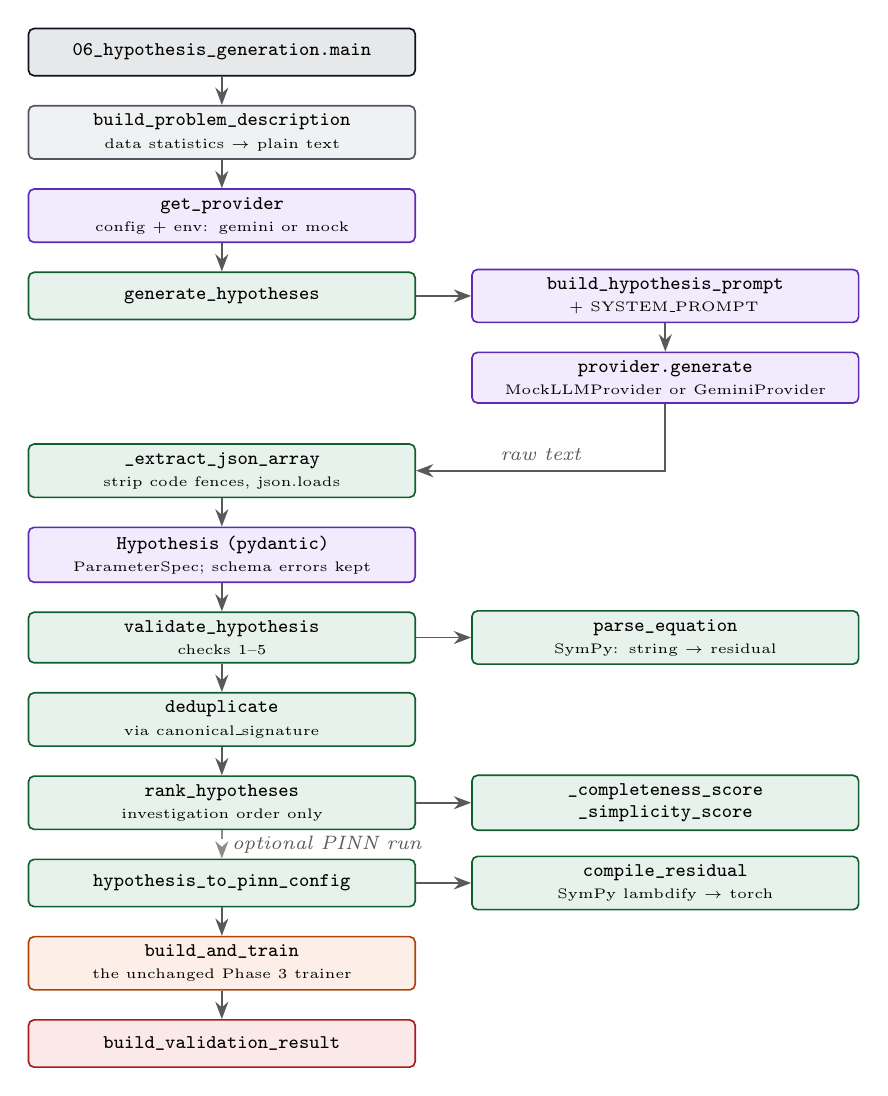
\begin{tikzpicture}[node distance=3.6mm and 7mm]
  \node[fnw=cExp] (main) {06_hypothesis_generation.main};
  \node[fnw=cData, below=of main] (desc) {build_problem_description\\{\normalfont\tiny data statistics $\to$ plain text}};
  \node[fnw=cLlm, below=of desc] (gp) {get_provider\\{\normalfont\tiny config + env: gemini or mock}};
  \node[fnw=cHyp, below=of gp] (gen) {generate_hypotheses};
  \node[fnw=cLlm, right=of gen] (prompt) {build_hypothesis_prompt\\{\normalfont\tiny + SYSTEM\_PROMPT}};
  \node[fnw=cLlm, below=of prompt] (call) {provider.generate\\{\normalfont\tiny MockLLMProvider or GeminiProvider}};
  \node[fnw=cHyp, below=of gen, yshift=-12mm] (json) {_extract_json_array\\{\normalfont\tiny strip code fences, json.loads}};
  \node[fnw=cLlm, below=of json] (schema) {Hypothesis (pydantic)\\{\normalfont\tiny ParameterSpec; schema errors kept}};
  \node[fnw=cHyp, below=of schema] (val) {validate_hypothesis\\{\normalfont\tiny checks 1--5}};
  \node[fnw=cHyp, right=of val] (parse) {parse_equation\\{\normalfont\tiny SymPy: string $\to$ residual}};
  \node[fnw=cHyp, below=of val] (dedup) {deduplicate\\{\normalfont\tiny via canonical\_signature}};
  \node[fnw=cHyp, below=of dedup] (rank) {rank_hypotheses\\{\normalfont\tiny investigation order only}};
  \node[fnw=cHyp, right=of rank] (scores) {_completeness_score\\_simplicity_score};
  \node[fnw=cHyp, below=of rank] (adapt) {hypothesis_to_pinn_config};
  \node[fnw=cHyp, right=of adapt] (comp) {compile_residual\\{\normalfont\tiny SymPy lambdify $\to$ torch}};
  \node[fnw=cPinn, below=of adapt] (train) {build_and_train\\{\normalfont\tiny the unchanged Phase 3 trainer}};
  \node[fnw=cVal, below=of train] (score) {build_validation_result};
  \draw[flow] (main) -- (desc); \draw[flow] (desc) -- (gp); \draw[flow] (gp) -- (gen);
  \draw[flow] (gen) -- (prompt); \draw[flow] (prompt) -- (call);
  \draw[flow] (call) |- node[note, above, pos=0.75]{raw text} (json);
  \draw[flow] (json) -- (schema); \draw[flow] (schema) -- (val); \draw[flow] (val) -- (parse);
  \draw[flow] (val) -- (dedup); \draw[flow] (dedup) -- (rank); \draw[flow] (rank) -- (scores);
  \draw[dflow] (rank) -- node[note, right]{optional PINN run} (adapt);
  \draw[flow] (adapt) -- (comp); \draw[flow] (adapt) -- (train); \draw[flow] (train) -- (score);
\end{tikzpicture}
\pkglegend
\caption{Hypothesis generation, deterministic validation and compilation into a PINN.}\end{figure}

\begin{figure}[!htb]\centering% flowchart 'p5' -- shared by project_guide.tex and submission_report.tex
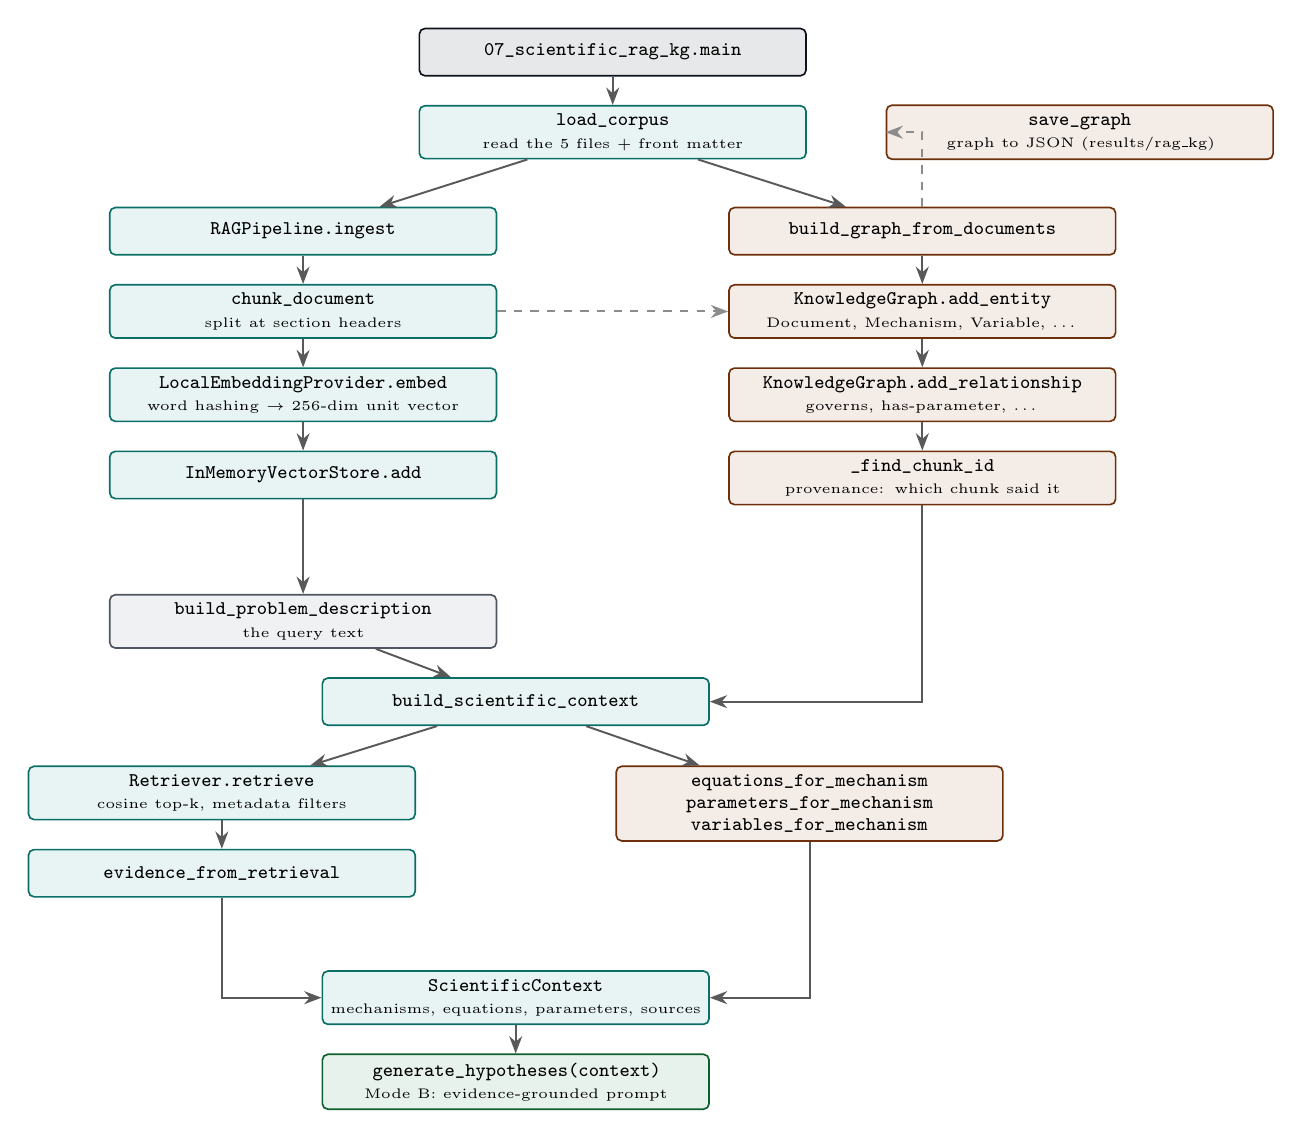
\begin{tikzpicture}[node distance=3.6mm and 6mm]
  \node[fnw=cExp] (main) {07_scientific_rag_kg.main};
  \node[fnw=cRag, below=of main] (lc) {load_corpus\\{\normalfont\tiny read the 5 files + front matter}};
  % RAG column (left)
  \node[fnw=cRag, below left=6mm and -10mm of lc] (ing) {RAGPipeline.ingest};
  \node[fnw=cRag, below=of ing] (chunk) {chunk_document\\{\normalfont\tiny split at section headers}};
  \node[fnw=cRag, below=of chunk] (emb) {LocalEmbeddingProvider.embed\\{\normalfont\tiny word hashing $\to$ 256-dim unit vector}};
  \node[fnw=cRag, below=of emb] (vs) {InMemoryVectorStore.add};
  % KG column (right)
  \node[fnw=cKg, below right=6mm and -10mm of lc] (bg) {build_graph_from_documents};
  \node[fnw=cKg, below=of bg] (ent) {KnowledgeGraph.add_entity\\{\normalfont\tiny Document, Mechanism, Variable, \ldots}};
  \node[fnw=cKg, below=of ent] (rel) {KnowledgeGraph.add_relationship\\{\normalfont\tiny governs, has-parameter, \ldots}};
  \node[fnw=cKg, below=of rel] (src) {_find_chunk_id\\{\normalfont\tiny provenance: which chunk said it}};
  % merge
  \node[fnw=cData, below=12mm of vs] (pd) {build_problem_description\\{\normalfont\tiny the query text}};
  \node[fnw=cRag, below=of pd, xshift=27mm] (ctx) {build_scientific_context};
  \node[fnw=cRag, below left=5mm and -12mm of ctx] (ret) {Retriever.retrieve\\{\normalfont\tiny cosine top-k, metadata filters}};
  \node[fnw=cRag, below=of ret] (ev) {evidence_from_retrieval};
  \node[fnw=cKg, below right=5mm and -12mm of ctx] (q) {equations_for_mechanism\\parameters_for_mechanism\\variables_for_mechanism};
  \node[fnw=cRag, below=31mm of ctx] (sc) {ScientificContext\\{\normalfont\tiny mechanisms, equations, parameters, sources}};
  \node[fnw=cHyp, below=of sc] (gen) {generate_hypotheses(context)\\{\normalfont\tiny Mode B: evidence-grounded prompt}};
  \node[fnw=cKg, right=of lc, xshift=4mm] (ser) {save_graph\\{\normalfont\tiny graph to JSON (results/rag\_kg)}};
  \draw[flow] (main) -- (lc); \draw[flow] (lc) -- (ing); \draw[flow] (lc) -- (bg);
  \draw[flow] (ing) -- (chunk); \draw[flow] (chunk) -- (emb); \draw[flow] (emb) -- (vs);
  \draw[flow] (bg) -- (ent); \draw[flow] (ent) -- (rel); \draw[flow] (rel) -- (src);
  \draw[dflow] (chunk.east) -- (bg.west |- chunk.east);
  \draw[dflow] (bg.north) |- (ser.west);
  \draw[flow] (vs) -- (pd); \draw[flow] (pd) -- (ctx); \draw[flow] (src) |- (ctx);
  \draw[flow] (ctx) -- (ret); \draw[flow] (ret) -- (ev); \draw[flow] (ctx) -- (q);
  \draw[flow] (ev) |- (sc); \draw[flow] (q) |- (sc); \draw[flow] (sc) -- (gen);
\end{tikzpicture}
\pkglegend
\caption{Scientific RAG and knowledge-graph construction into one scientific context.}\end{figure}

\begin{figure}[!htb]\centering% flowchart 'p7' -- shared by project_guide.tex and submission_report.tex
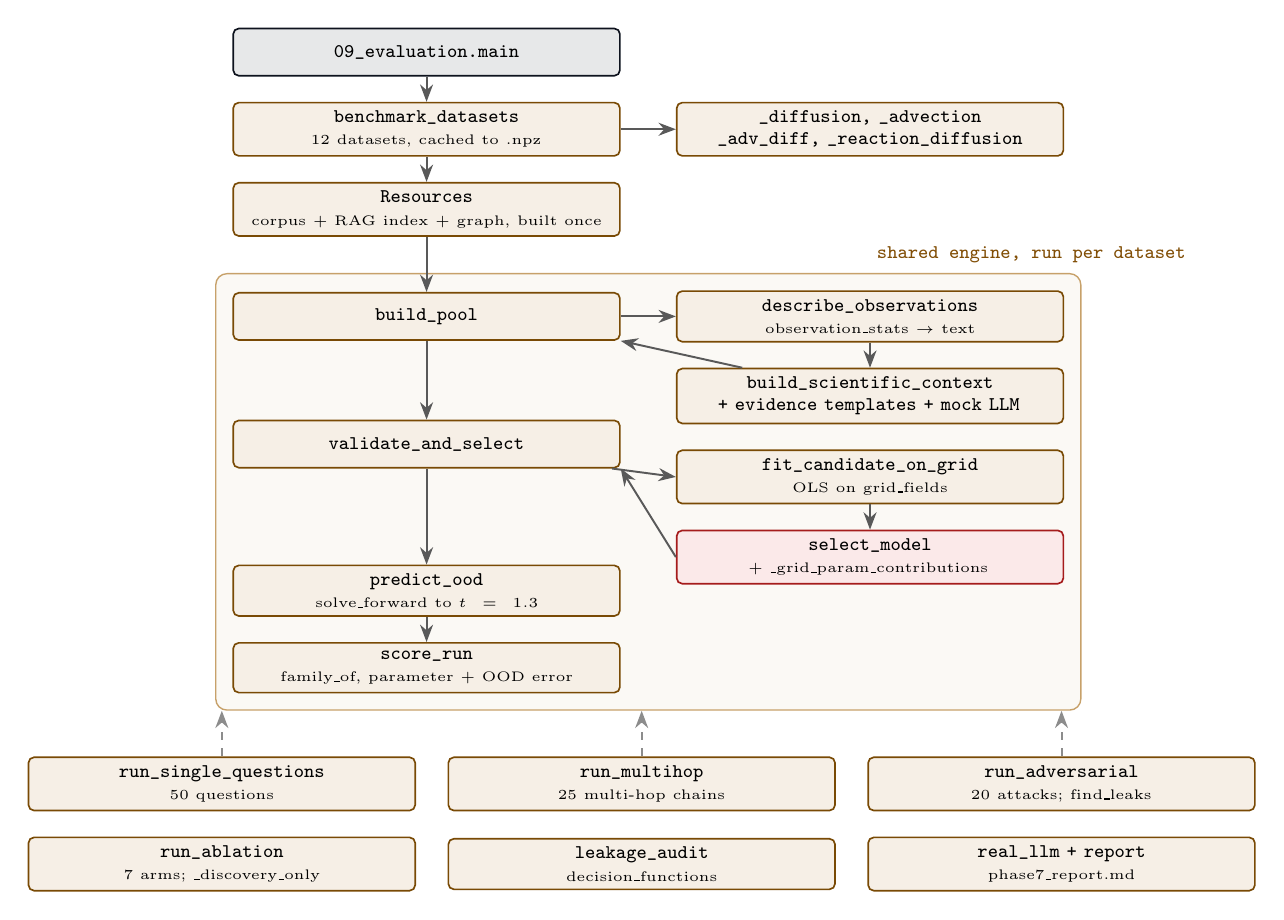
\begin{tikzpicture}[node distance=3.2mm and 7mm]
  \node[fnw=cExp] (main) {09_evaluation.main};
  \node[fnw=cEval, below=of main] (ds) {benchmark_datasets\\{\normalfont\tiny 12 datasets, cached to .npz}};
  \node[fnw=cEval, right=of ds] (mk) {_diffusion, _advection\\_adv_diff, _reaction_diffusion};
  \node[fnw=cEval, below=of ds] (res) {Resources\\{\normalfont\tiny corpus + RAG index + graph, built once}};
  \node[fnw=cEval, below=7mm of res] (bp) {build_pool};
  \node[fnw=cEval, right=of bp] (dsc) {describe_observations\\{\normalfont\tiny observation_stats $\to$ text}};
  \node[fnw=cEval, below=of dsc] (ctx) {build_scientific_context\\+ evidence templates + mock LLM};
  \node[fnw=cEval, below=10mm of bp] (vs) {validate_and_select};
  \node[fnw=cEval, below=of ctx] (fit) {fit_candidate_on_grid\\{\normalfont\tiny OLS on grid_fields}};
  \node[fnw=cVal, below=of fit] (sm) {select_model\\{\normalfont\tiny + _grid_param_contributions}};
  \node[fnw=cEval, below=of vs, yshift=-9mm] (ood) {predict_ood\\{\normalfont\tiny solve_forward to $t=1.3$}};
  \node[fnw=cEval, below=of ood] (sc) {score_run\\{\normalfont\tiny family_of, parameter + OOD error}};
  \begin{scope}[on background layer]
    \node[pkgbox=cEval, fit=(bp)(dsc)(sm)(sc), label={[pkglabel=cEval]above right:shared engine, run per dataset}] (eng) {};
  \end{scope}
  % suites
  \node[fnw=cEval, below=8mm of sc, xshift=-26mm] (s1) {run_single_questions\\{\normalfont\tiny 50 questions}};
  \node[fnw=cEval, right=4mm of s1] (s2) {run_multihop\\{\normalfont\tiny 25 multi-hop chains}};
  \node[fnw=cEval, right=4mm of s2] (s3) {run_adversarial\\{\normalfont\tiny 20 attacks; find_leaks}};
  \node[fnw=cEval, below=of s1] (s4) {run_ablation\\{\normalfont\tiny 7 arms; _discovery_only}};
  \node[fnw=cEval, right=4mm of s4] (s5) {leakage_audit\\{\normalfont\tiny decision_functions}};
  \node[fnw=cEval, right=4mm of s5] (s6) {real_llm + report\\{\normalfont\tiny phase7_report.md}};
  \draw[flow] (main) -- (ds); \draw[flow] (ds) -- (mk); \draw[flow] (ds) -- (res); \draw[flow] (res) -- (bp);
  \draw[flow] (bp) -- (dsc); \draw[flow] (dsc) -- (ctx); \draw[flow] (ctx) -- (bp.south east);
  \draw[flow] (bp) -- (vs); \draw[flow] (vs) -- (fit.west); \draw[flow] (fit) -- (sm); \draw[flow] (sm.west) -- (vs.south east);
  \draw[flow] (vs) -- (ood); \draw[flow] (ood) -- (sc);
  \draw[dflow] (s1.north) -- (s1.north |- eng.south);
  \draw[dflow] (s2.north) -- (s2.north |- eng.south);
  \draw[dflow] (s3.north) -- (s3.north |- eng.south);
\end{tikzpicture}
\pkglegend
\caption{Benchmark, adversarial, ablation and leakage evaluation.}\end{figure}

\begin{figure}[!htb]\centering% flowchart 'gemini' -- used by docs/Report.tex
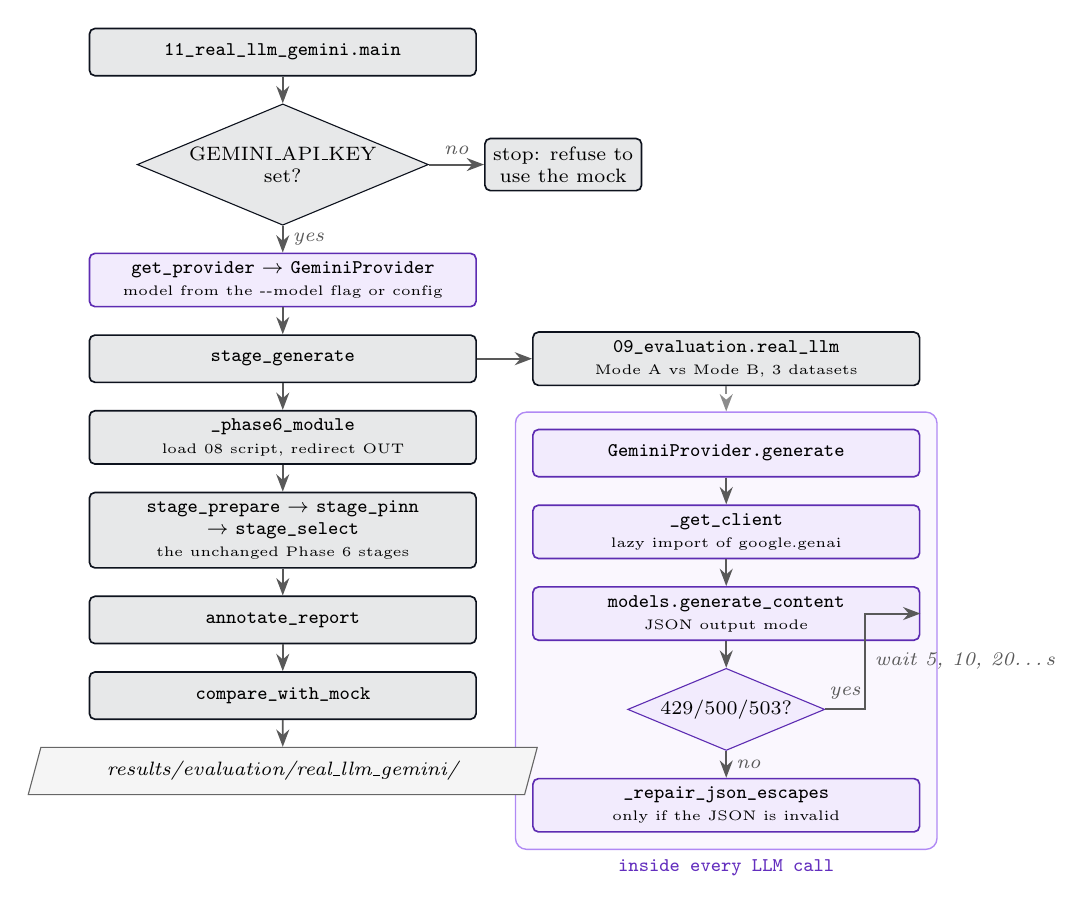
\begin{tikzpicture}[node distance=3.4mm and 7mm]
  \node[fnw=cExp] (main) {11_real_llm_gemini.main};
  \node[dec=cExp, below=of main] (key) {GEMINI_API_KEY\\set?};
  \node[fn=cExp, right=of key, font=\scriptsize] (stop) {stop: refuse to\\use the mock};
  \node[fnw=cLlm, below=of key] (gp) {get_provider $\to$ GeminiProvider\\{\normalfont\tiny model from the -{}-model flag or config}};
  \node[fnw=cExp, below=of gp] (sg) {stage_generate};
  \node[fnw=cExp, right=of sg] (rl) {09_evaluation.real_llm\\{\normalfont\tiny Mode A vs Mode B, 3 datasets}};
  \node[fnw=cExp, below=of sg] (p6) {_phase6_module\\{\normalfont\tiny load 08 script, redirect OUT}};
  \node[fnw=cExp, below=of p6] (st) {stage_prepare $\to$ stage_pinn\\$\to$ stage_select\\{\normalfont\tiny the unchanged Phase 6 stages}};
  \node[fnw=cExp, below=of st] (ar) {annotate_report};
  \node[fnw=cExp, below=of ar] (cm) {compare_with_mock};
  \node[io, below=of cm] (out) {results/evaluation/real\_llm\_gemini/};
  % provider internals
  \node[fnw=cLlm, right=of p6, yshift=-2mm] (gen) {GeminiProvider.generate};
  \node[fnw=cLlm, below=of gen] (cl) {_get_client\\{\normalfont\tiny lazy import of google.genai}};
  \node[fnw=cLlm, below=of cl] (gc) {models.generate_content\\{\normalfont\tiny JSON output mode}};
  \node[dec=cLlm, below=of gc] (err) {429/500/503?};
  \node[fnw=cLlm, below=of err] (rep) {_repair_json_escapes\\{\normalfont\tiny only if the JSON is invalid}};
  \begin{scope}[on background layer]
    \node[pkgbox=cLlm, fit=(gen)(cl)(gc)(err)(rep), label={[pkglabel=cLlm]below:inside every LLM call}] (box) {};
  \end{scope}
  \draw[flow] (main) -- (key); \draw[flow] (key) -- node[note, above]{no} (stop);
  \draw[flow] (key) -- node[note, right]{yes} (gp); \draw[flow] (gp) -- (sg); \draw[flow] (sg) -- (rl);
  \draw[flow] (sg) -- (p6); \draw[flow] (p6) -- (st); \draw[flow] (st) -- (ar); \draw[flow] (ar) -- (cm);
  \draw[flow] (cm) -- (out);
  \draw[flow] (gen) -- (cl); \draw[flow] (cl) -- (gc); \draw[flow] (gc) -- (err);
  \draw[flow] (err.east) -- node[note, above]{yes} ++(5mm,0) |- node[note, right, pos=0.25]{wait 5, 10, 20\ldots s} (gc.east);
  \draw[flow] (err) -- node[note, right]{no} (rep);
  \draw[dflow] (rl.south) -- (box.north -| rl.south);
\end{tikzpicture}
\pkglegend
\caption{Real-LLM (Gemini) run and the provider's retry/JSON handling.}\end{figure}

\end{document}
